\chapter{Introduction}
\section{Context and motivation}
Digital signatures are an integral part of secure communication today. They enable a receiver of a digital message to mathematically verify the sender is who they say they are. 
The widely used \gls{dsa} and the \gls{rsa} 
signature scheme are in peril due to the potential emergence of quantum computers which can break the hard problems \gls{dsa} and \gls{rsa}-sign are based upon.
Whether practical quantum computers with these powers will emerge any time soon is debatable. However, measures against the looming threat has already begun. 
In 2016, the \gls{nist} announced a process for selecting new standard schemes for \gls{kems} and 
digital signatures that are resilient against quantum attacks (https://www.nist.gov/pqcrypto). Many of the submissions to this process, including KRYSTALS-Dilithium which is to be standardized, 
are based on lattice problems that are believed to be hard to solve for both classical and quantum computers.

Cryptographic schemes based on lattice problems are not an entirely new phenomenon, however. NTRU-Sign \cite{NTRUSign03}, the signature counterpart of the NTRU crypto-system,
is a digital signature scheme based on the hardness of the \gls{cvp}, a well known lattice problem (source?).
The original scheme was broken by Phong. Q. Nguyen \& Oded Regev in 2006 \cite{NR09}; not by solving the \gls{cvp}, but by retrieving a secret key by observing enough signatures.
In other words, each signature leaks some information about the secret key.
The title of their paper and the name of the attack is \textit{Learning a Parallelepiped}, and the problem to solve in this attack will henceforth be denoted as the \gls{hpp} as one tries to \textit{learn} a parallelepiped.
Countermeasures for this attack was proposed, but ultimately broken again in 2012 due to a more advanced extension of the original attack \cite{Zonotope12}.

Hawk \cite{HawkSpec24} is a digital signature scheme submitted to NIST's standardization process and is a viable candidate for standardization
due to its speed and small signature- and keysizes. This thesis will investigate if a method based on \gls{hpp} can be aimed at
Hawk to retrieve information about the secret key.
% It has some notable structural similarities to that of NTRUsign, but is theoretically safe from the \gls{hpp} attack.
% In practice, however, this might not necessarily be the case. 

\section{Objectives}
The objective of this thesis consists of two main parts:
\begin{itemize}
    \item \textbf{Implementation of Hawk in Rust}. As the first part of this thesis I implement the Hawk digital signature scheme according to \cite{HawkSpec24} in the Rust programming language. 
    Implementing a scheme and its algorithms is a good way to more deeply learn how it works. I chose to implement it in Rust for the sake of learning the language as a personal bonus objective of the thesis.
    Moreover, having ones own version of an algorithm makes it easier to experiment, run simulations, adjust, and modify it to ones need. It would in any case be challenging to understand and work with dense, long, 
    and complicated source code someone else has written. For the Hawk teams source code and reference implementation see https://github.com/hawk-sign.

    Disclaimer: this implementation is not meant to be comparable with the Hawk teams implementation for real life usage, as it is not highly optimized and not all formal requirements are met.

\item \textbf{Cryptanalysis and experimentation}. The second part of this thesis is cryptanalysis of Hawk. The goal is to use the \textit{Learning a parallelepiped} attack and adjusting it to attack Hawk. 
    This requires both theoretical and practical work, and experiments will, like the Hawk implementation itself, be implemented in Rust.
\end{itemize}
\section{Thesis outline}
Chapter 2 will introduce important notions and mathematical background used in this thesis. Chapter 3 will introduce Hawk and its implementation, and the \textit{Learning a Parallelepiped} attack.
In Chapter 4 the cryptanalysis of Hawk is presented. The final chapter will discuss results and future work.


\subsection{Listings}
You can do listings, like in Listing~\ref{ListingReference}
\begin{lstlisting}[caption={[Short caption]Look at this cool listing. Find the rest in Appendix~\ref{Listing}},label=ListingReference]
$ java -jar myAwesomeCode.jar
\end{lstlisting}

You can also do language highlighting for instance with Golang:
And in line~\ref{LineThatDoesSomething} of Listing~\ref{ListingGolang} you can see that we can ref to lines in listings.

\begin{lstlisting}[caption={Hello world in Golang},label=ListingGolang,escapechar=|]
package main

import "fmt"

func main() {
    fmt.Println("hello world") |\label{LineThatDoesSomething}|
}

\end{lstlisting}

\subsection{Figures}

Example of a centred figure
\begin{figure}[H]
    \centering
    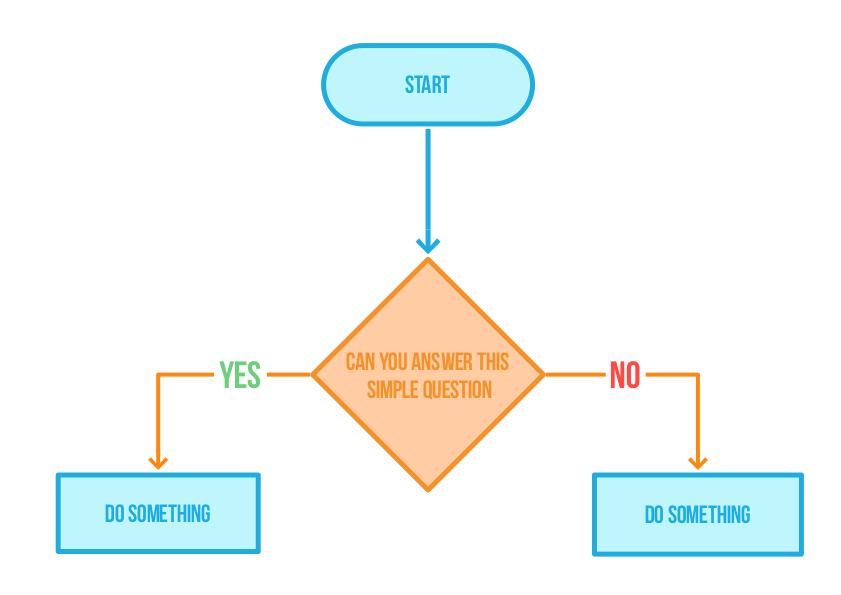
\includegraphics[scale=0.5]{figures/Flowchart}
    \caption{Caption for flowchart}
  	\medskip 
	\hspace*{15pt}\hbox{\scriptsize Credit: Acme company makes everything \url{https://acme.com/}}
    \label{FlowchartFigure}
\end{figure}

\subsection{Tables}

We can also do tables. Protip: use \url{https://www.tablesgenerator.com/} for generating tables.
\begin{table}[H]
\centering
\caption{Caption of table}
\label{TableLabel}
\begin{tabular}{|l|l|l|}
\hline
Title1 & Title2 & Title3 \\ \hline
data1  & data2  & data3  \\ \hline
\end{tabular}
\end{table}

\subsection{\gls{git}}

\gls{git} is fun, use it!
